\documentclass[../root.tex]{subfiles}

\begin{document}

\section{Rationale}

The methods presented in the previous Chapter work with general domains. However,
we can take advantage of the structure of our particular problem. The key observation
is that the robot can focus on retrieving one of the components, forgetting about the
unrelated ones. That is, the planning problem can be simplified in the presence of
precedence relationships.

The main source of precedence in our case is partial occlusion. If a component occludes
another, it is a good candidate to be removed first. Even if it is possible to remove
an occluded component, removing first the occluding object can lead to the discovery
of a better affordance than those that have already been detected.
Therefore, a good strategy to gain in computational efficiency and to increase the
chances of success is to
perform topological sorting based on precedence relations, and disassemble first the
components with no precedences. The predicates that are not directly related to this
component can be removed from the state, easing the task for the planner.
That is, we want to enable the robot to focus its attention on a particular component
of the device. In this Chapter we consider the problem in its full form: the device
is composed of components that may hide each other. While some precedence relations
are observable (e.g. \texttt{(partially-occludes ...)}), others are not (e.g.
a hidden screw fixing a component on the other side). It is our intention to deal
successfully with both kind of precedences.

\section{Simplifying the state}

Let us consider an hypothetical hard drive scenario in which the lid and the PCB have already
been removed. The only remaining components left to extract are the reader and the platter.
The reader is fixed by a screw on the other side, and at the same time is occluding part
of the platter. It turns out that the reader is hiding a high quality suction point. This
scenario has been represented as a graph in Fig.~\ref{fig:device}. This kind of representation
is useful to represent graphically the distribution of the components, and to operate with
its topological properties. Of course, the robot would not see the hidden features, so it would
be restricted to the view of Fig.~\ref{fig:simple-device-no-hidden}.

\begin{figure}[tbhp]
	\centering
	\begin{subfigure}[b]{0.77\columnwidth}
		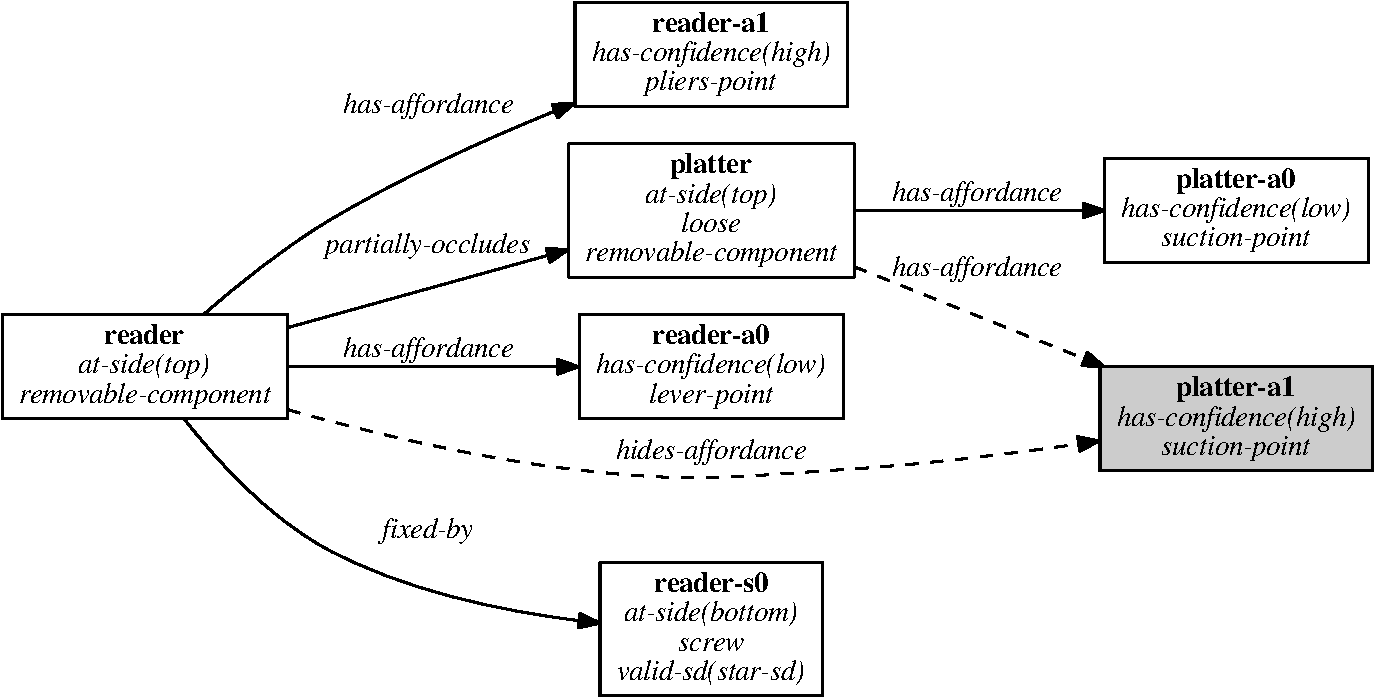
\includegraphics[width=\textwidth]{simple-device-crop}
		\caption{}
		\label{fig:simple-device}
	\end{subfigure}

	\vspace{0.5cm}

	\begin{subfigure}[b]{0.75\columnwidth}
		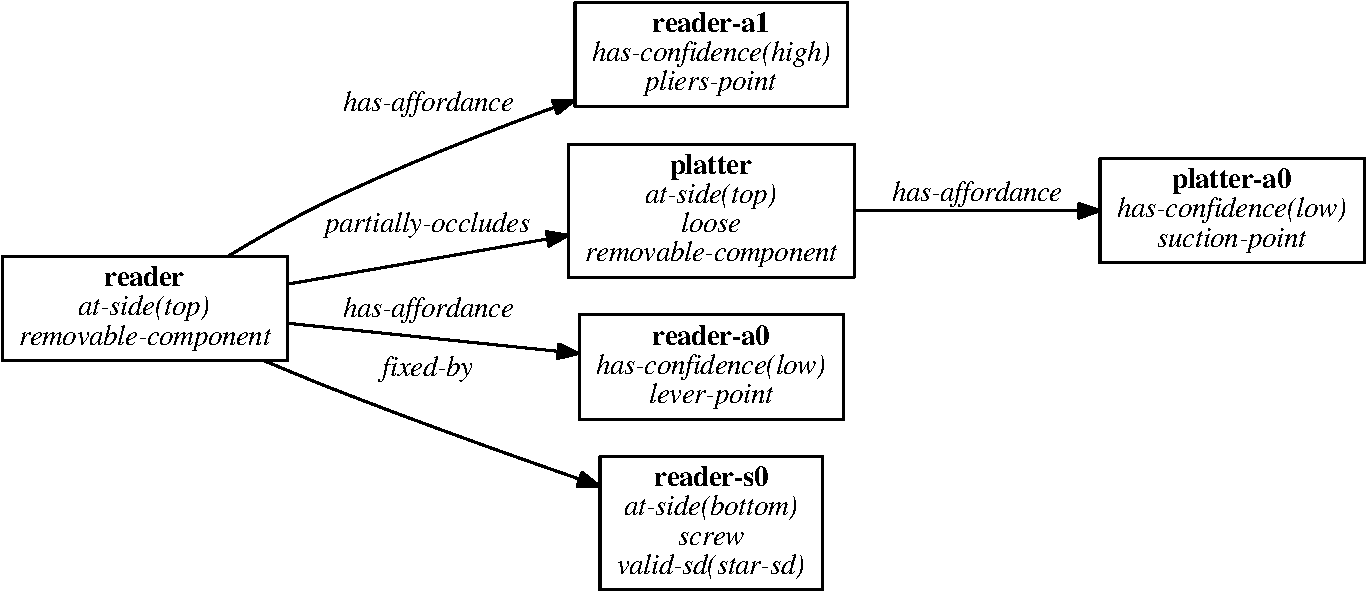
\includegraphics[width=\textwidth]{simple-device-no-hidden-crop}
		\caption{}
		\label{fig:simple-device-no-hidden}
	\end{subfigure}

	\vspace{0.5cm}

	\begin{subfigure}[b]{0.60\columnwidth}
		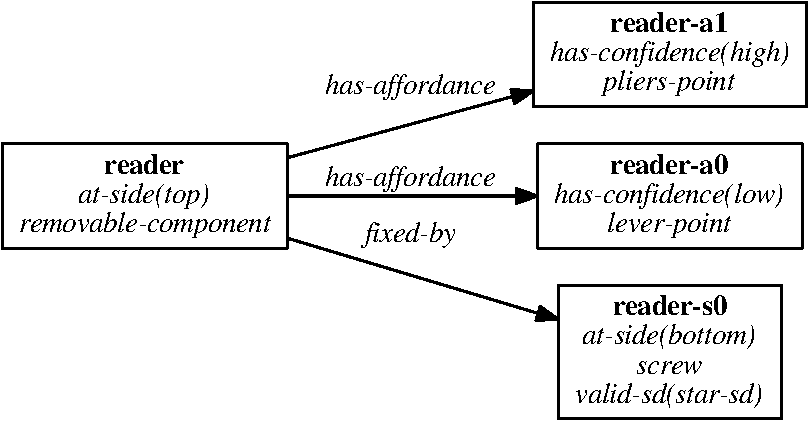
\includegraphics[width=\textwidth]{simple-device-no-occlusions-crop}
		\caption{}
		\label{fig:simple-device-no-occlusions}
	\end{subfigure}
	\caption{
		(a) Simple hard drive scenario. The hidden nodes are shaded in gray,
			and the hidden relations are represented as dashed edges.
		(b) The state that the robot would actually see (i.e. without the
			hidden nodes/edges).
        (c) Simplified state after removing the partial occlusions: the platter
			and its only detected affordance have been removed. The robot can
			use this simplified state to focus on the removal of the reader.
	}
	\label{fig:device}
\end{figure}

Now, let us see that the robot could remove the platter much more efficiently if the reader
was out of the way. However, when a planner is fed with this state, it may determine that
it is better to remove the platter first (let us remember that the planner operates under
the assumption of full observability). However, we know that removing first the reader can
potentially lead to a much better scenario.

The strategy that we follow is to first identify the components without partial occlusions.
We select one of these components for removal (we show in the next Section the criterion
used to select the component). Then
we use breadth first search to identify the closest neighbors, since these are the ones that
are more prone to be relevant in the disassembly of the chosen component. When invoking
breadth first search, we do not navigate through the \texttt{partially-occluded} edges in order
to avoid the accidental inclusion of the components that we want to avoid. The result
of doing this in the state of Fig.~\ref{fig:simple-device-no-hidden} can be shown in
Fig.~\ref{fig:simple-device-no-occlusions}. This is, in fact, a form of hierarchical planning.
We sort the tasks according to their
precedences and solve them in order, without caring about the rest.

\section{Dealing with unseen precedences}

In the previous section we dealt with observable precedences. However, we can
expect to encounter situations such as the one from Fig.~\ref{fig:complex-device}.
In this particular scenario, the task that the robot has chosen to complete is impossible.
This is because it cannot possibly know that there is a hidden screw on the other side
of the hard disk keeping the reader in place. However, after a few trials, we can reasonably
assume that this task should be tried later.

When choosing one task to complete from the set of tasks with no visible precedences and
with no previous experience, the robot may choose any of them. However, if it fails many
times during the completion of the task, it can assume that it has picked the wrong
component to disassemble, and that it should try another task. The robot can return the
component back to the goal stack, and select another one.

We have implemented this feature giving a score to each component. Whenever the robot repeats
the same action several times with no success, we decrease the score of the component and
pick another available goal with a higher score.

\begin{figure}[tbhp]
	\centering
	\begin{subfigure}[b]{0.77\columnwidth}
		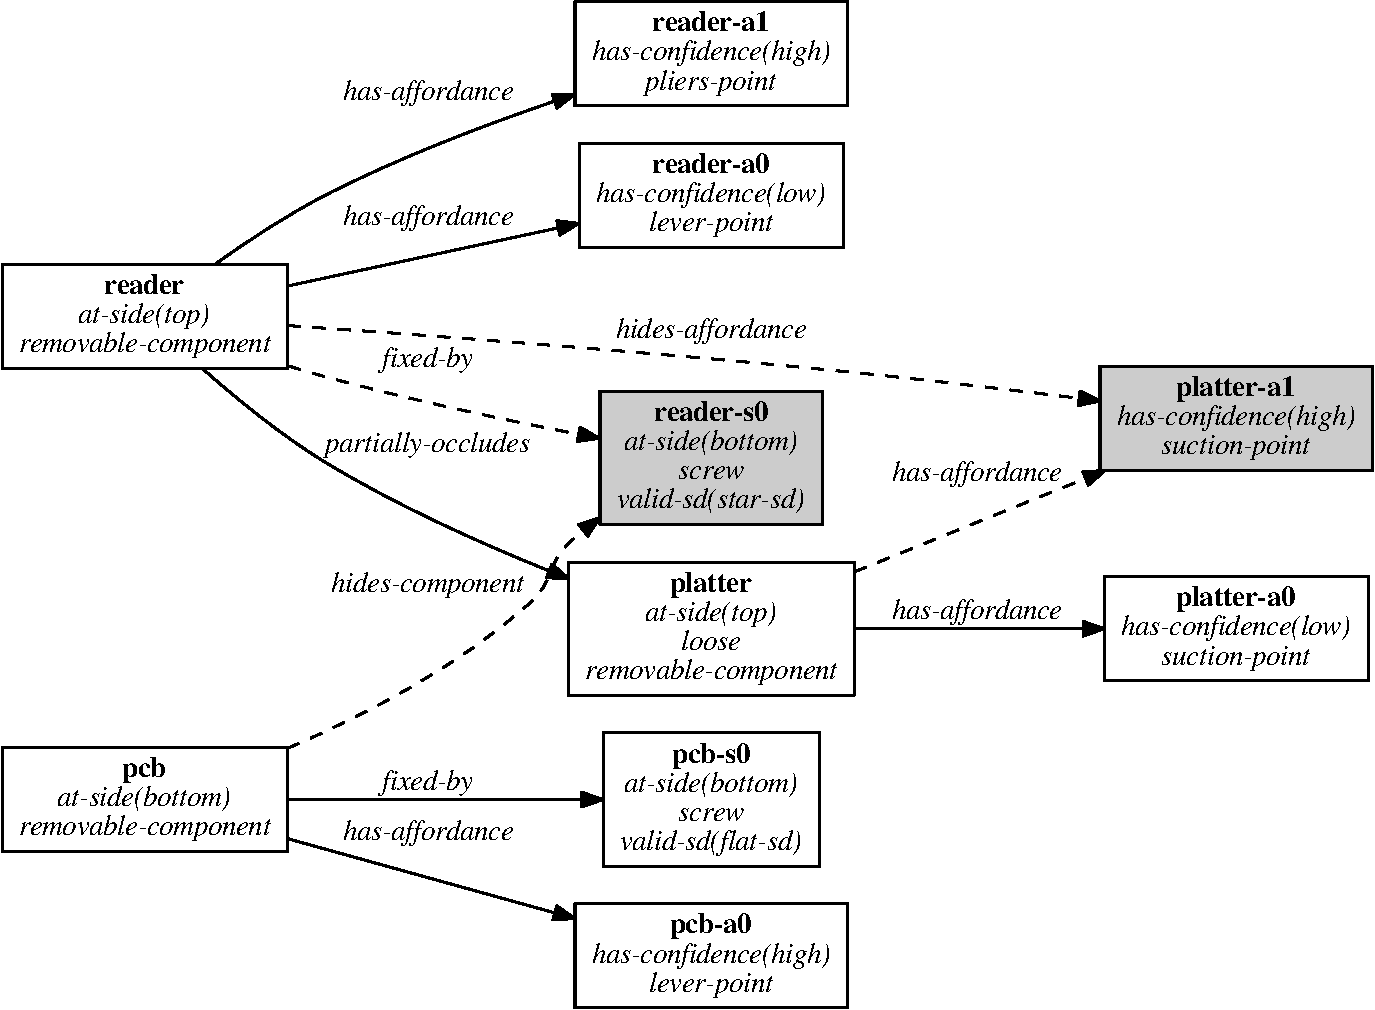
\includegraphics[width=\textwidth]{complex-device}
		\caption{}
		\label{fig:complex-device-all}
	\end{subfigure}

	\vspace{0.5cm}

	\begin{subfigure}[b]{0.75\columnwidth}
		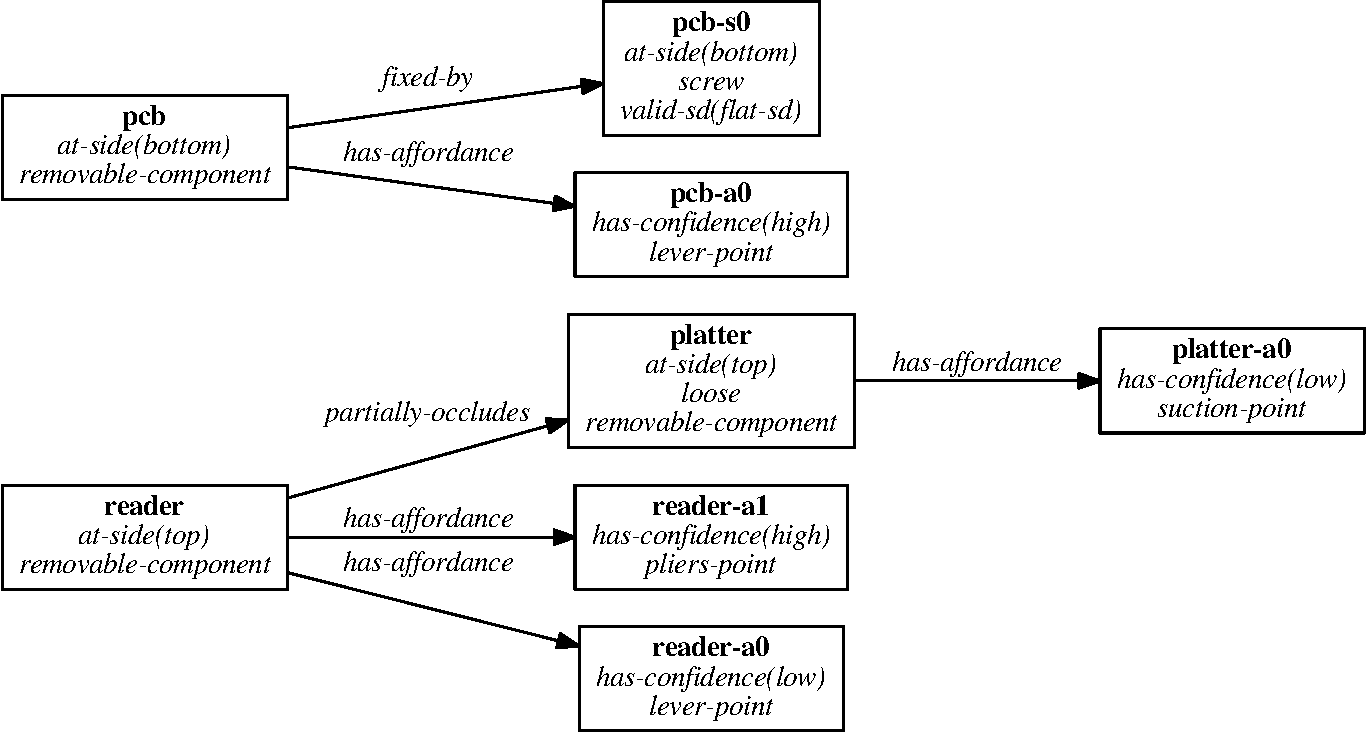
\includegraphics[width=\textwidth]{complex-device-no-hidden}
		\caption{}
		\label{fig:complex-device-no-hidden}
	\end{subfigure}

	\vspace{0.5cm}

	\begin{subfigure}[b]{0.60\columnwidth}
		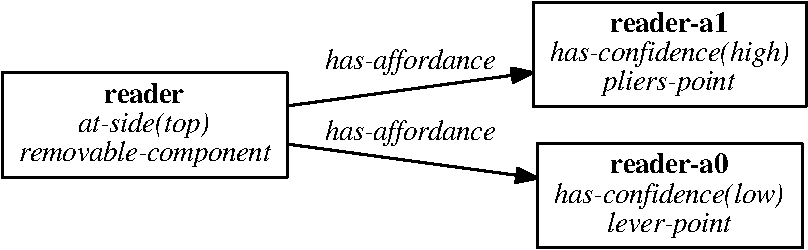
\includegraphics[width=\textwidth]{complex-device-no-occlusions}
		\caption{}
		\label{fig:complex-device-no-occlusions}
	\end{subfigure}
	\caption{
		(a) Complex distribution with one hidden precedence: there is one hidden
			screw below the PCB blocking the reader.
		(b) The state that the robot would actually see (i.e. without the
			hidden nodes/edges). Note that, in particular, the reader seems
			to have no precedence.
        (c) Simplified state after removing the partial occlusions, focused on the
			reader. The robot will never succeed removing the it.
	}
	\label{fig:complex-device}
\end{figure}

\IfEq{\jobname}{\detokenize{root}}{}{\printbibliography}

\end{document}